%%%%%%%%%%%%%%%%%%%%%%%%%%%%%%%%%%%%%%%%%
% Ay 190 - WS2
% Written by Chatarin Wong-u-railertkun
%%%%%%%%%%%%%%%%%%%%%%%%%%%%%%%%%%%%%%%%%

%----------------------------------------------------------------------------------------
%	PACKAGES AND OTHER DOCUMENT CONFIGURATIONS
%----------------------------------------------------------------------------------------

\documentclass[11pt,letterpaper]{article}

% Load some basic packages that are useful to have
% and that should be part of any LaTeX installation.
%

\usepackage{graphicx}     % be able to include figures

\usepackage{xcolor}         % get nice colors

% change default font to Palatino (looks nicer!)
\usepackage[latin1]{inputenc}
\usepackage{mathpazo}
\usepackage[T1]{fontenc}

% load some useful math symbols/fonts
\usepackage{latexsym,amsfonts,amsmath,amssymb}
\usepackage{subcaption}

% comfort package to easily set margins
\usepackage[top=1in, bottom=1in, left=1in, right=1in]{geometry}

% control some spacings
%
% spacing after a paragraph
\setlength{\parskip}{.15cm}
% indentation at the top of a new paragraph
\setlength{\parindent}{0.0cm}

\usepackage{courier}

%----------------------------------------------------------------------------------------
%	TITLE
%----------------------------------------------------------------------------------------

\begin{document}

\begin{center}
\Large
Ay190 -- Worksheet 03 \\    %%%%%% DON'T FORGET TO CHANGE THE WORK SHEET NUMBER
Chatarin (Mee) Wong-u-railertkun\\
Date: \today
\end{center}

%----------------------------------------------------------------------------------------
%	QUESTION 1
%----------------------------------------------------------------------------------------

\section{Integration via Newton-Cotes Formulae}

\subsection{Integration Over Sin(x) Function}

Do the numerical integration of sin(x) from x = 0 to x = $\pi$ with three different methods, midpoint, trapezoid, and Simpson's rule. The analytical answer is 2. Figure \ref{fig:ConvergentA} shows the absolute error. We can see that the error for midpoint and trapezoid method goes down quadratically, and error for SImpson's rule goes down with $h^4$, as expected.

\begin{figure}[h!]
	\centering
	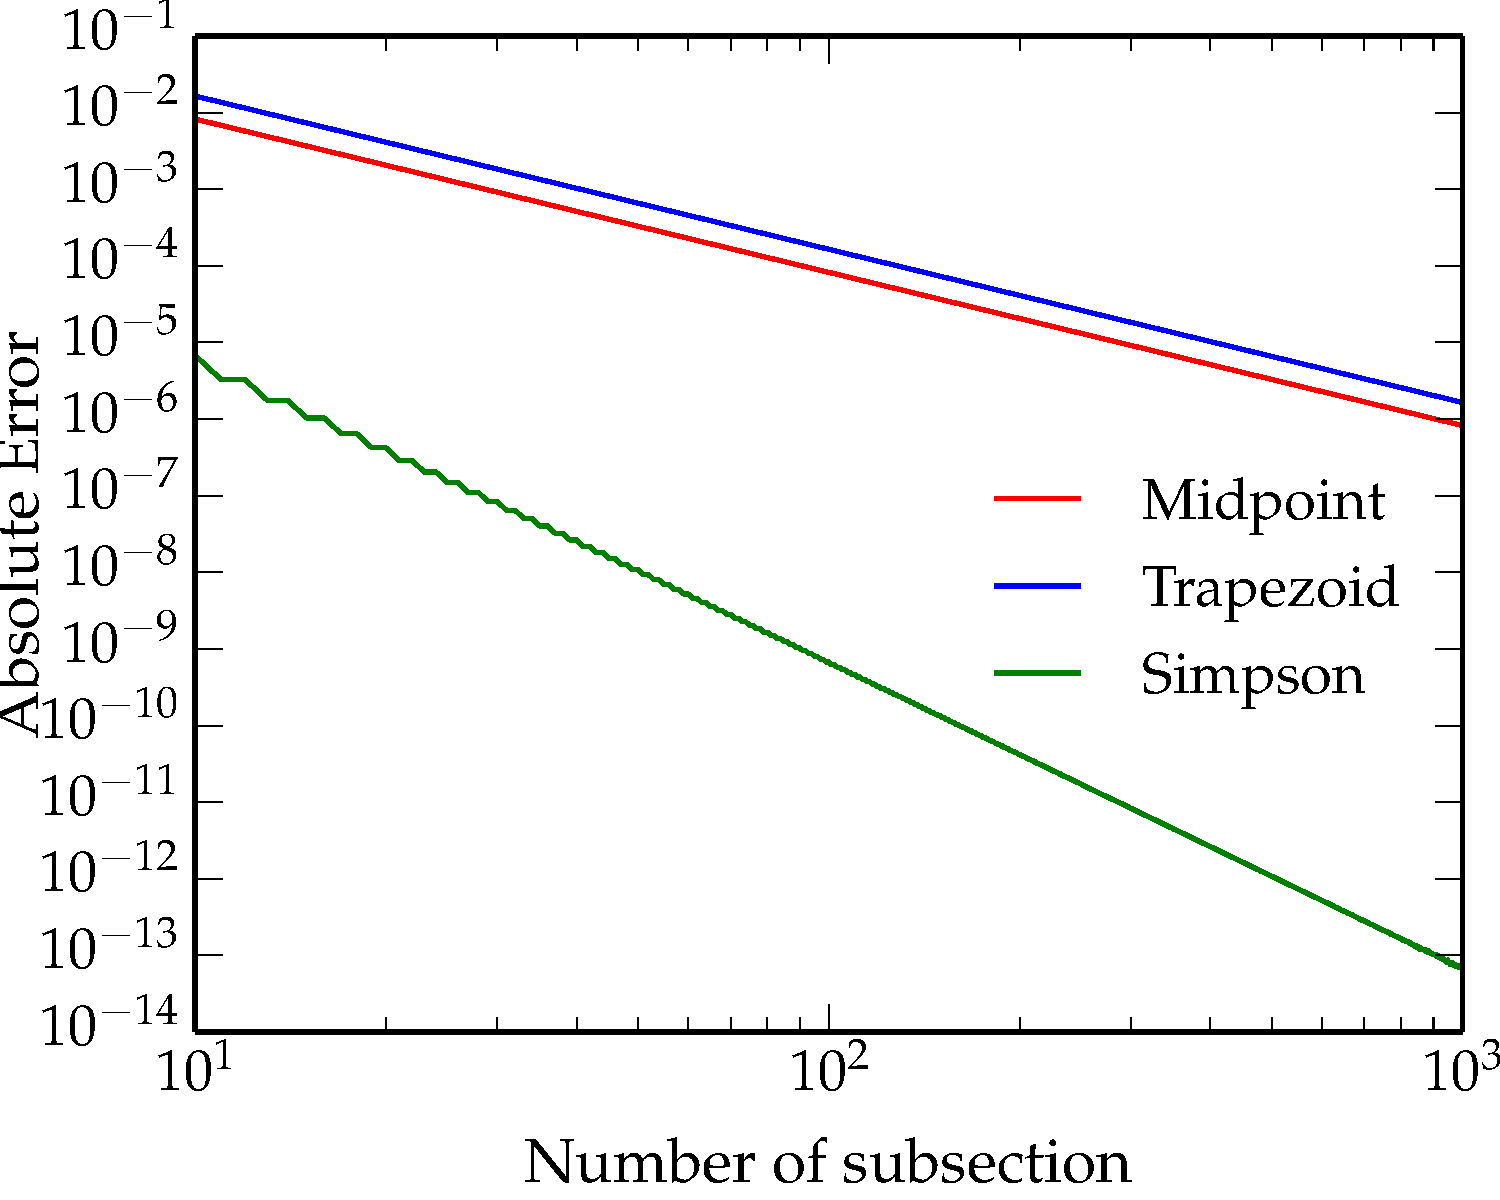
\includegraphics[width=0.5\textwidth]{ConvergentA}
	\caption{Absolute error from integration of sin(x) from x = 0 to x = $\pi$ with three different methods, midpoint, trapezoid, and Simpson's rule.}
	\label{fig:ConvergentA}
\end{figure}

\subsection{Integration Over x*Sin(x) Function}

Similar to above section, but now the integration is of x*sin(x) from x = 0 to x = $\pi$. Again, plot the absolute error to observe the convergent rate of three different methods. Figure \ref{fig:ConvergentB} show that the convergent rate (i.e. the slope of the line) is the same as in figure \ref{fig:ConvergentA}. 

\begin{figure}[h!]
	\centering
	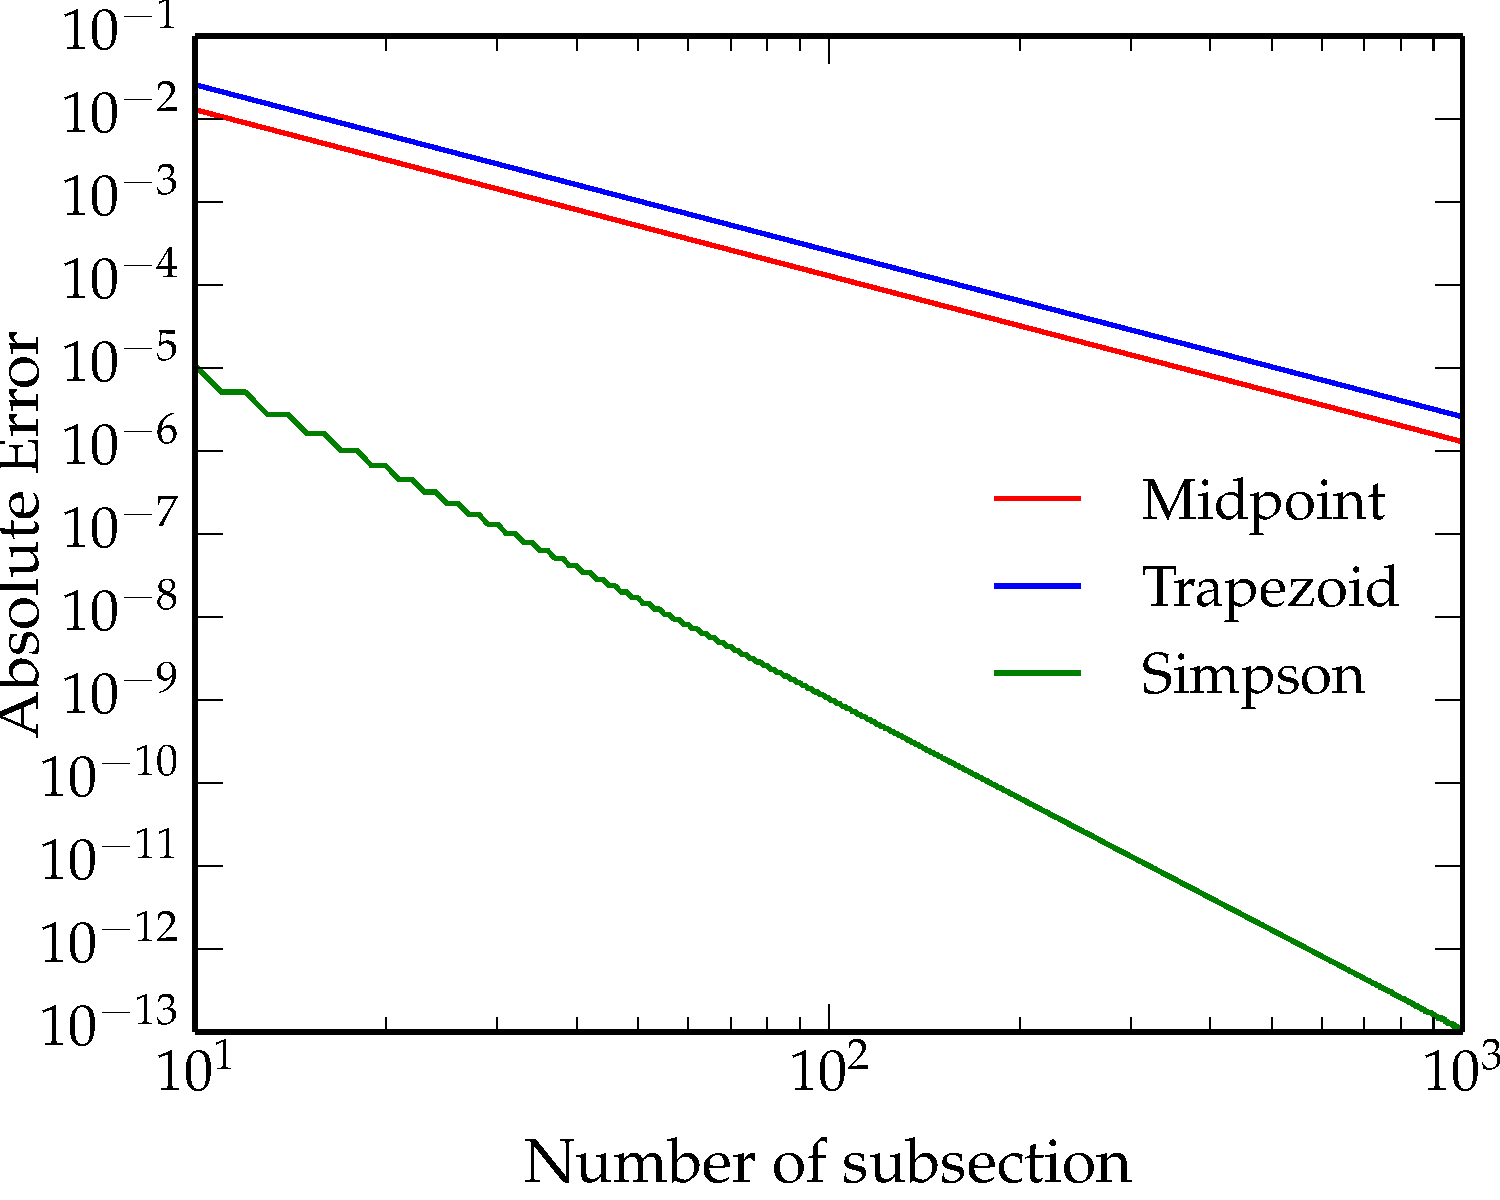
\includegraphics[width=0.5\textwidth]{ConvergentB}
	\caption{Absolute error from integration of x*sin(x) from x = 0 to x = $\pi$ with three different methods, midpoint, trapezoid, and Simpson's rule.}
	\label{fig:ConvergentB}
\end{figure}

%----------------------------------------------------------------------------------------
%	QUESTION 2
%----------------------------------------------------------------------------------------
\newpage
\section{Gaussian Quadrature}

\subsection{Gauss-Laguerre}

Modify the integral to get the correct weight function for the Gauss-Laguerre quadrature.

\begin{align*}
n_{e^{\pm}} &= \frac{8\pi(k_B T)^3}{(2\pi \bar{h} c)^3} \int_{0}^{\infty} \frac{x^2}{e^x+1}dx \\
                    &= \frac{8\pi(k_B T)^3}{(2\pi \bar{h} c)^3} \int_{0}^{\infty} \frac{1}{e^x} \frac{e^x x^2}{e^x+1}dx \\
                    &= \frac{8\pi(k_B T)^3}{(2\pi \bar{h} c)^3} \int_{0}^{\infty} W(x) \frac{e^x x^2}{e^x+1}dx
\end{align*}

The constant in front of the integral is approximately $8.4384 \times 10^{33} m^{-3}$. In figure \ref{fig:NumDens}, it seems that our answer is bounded by accuracy, even at low n. In fact, when I try to use high n as 500, python spits out an overflow error.

\begin{figure}[h!]
	\centering
	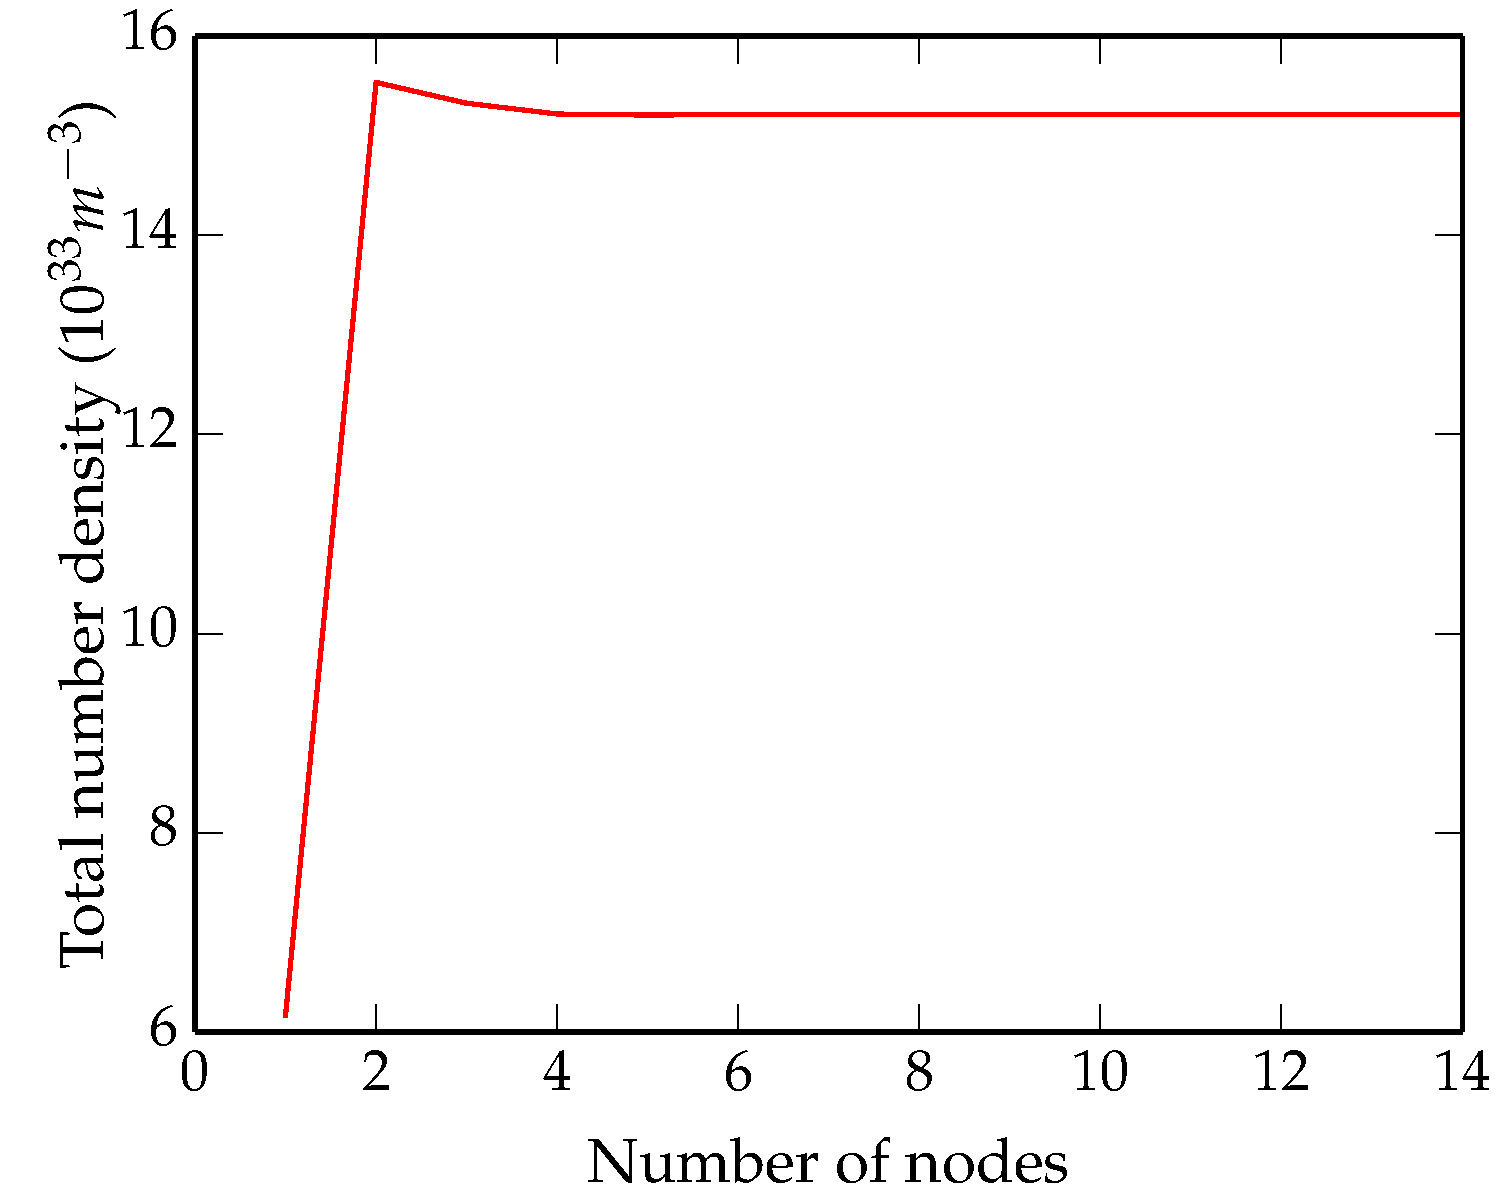
\includegraphics[width=0.5\textwidth]{NumDens}
	\caption{The number density calculated with different number of nodes of Laguerre function.}
	\label{fig:NumDens}
\end{figure}

\subsection{Gauss-Legendre}

Modify the integral in terms of energy, $E=pc$, by substitute $x=\beta E$.

\begin{align*}
n_{e^{\pm}} &= \frac{8\pi(k_B T)^3}{(2\pi \bar{h} c)^3} \int_{0}^{\infty} \frac{x^2}{e^x+1}dx \\
                    &= \frac{8\pi}{(2\pi \bar{h} c)^3} \int_{0}^{\infty} \frac{E^2}{e^{\beta E}+1}dE \\
\end{align*}

We shall divide the integral into bins, with width of $\Delta E=5MeV$, up until $E \approx 150 MeV$.

\begin{figure}[h!]
	\centering
	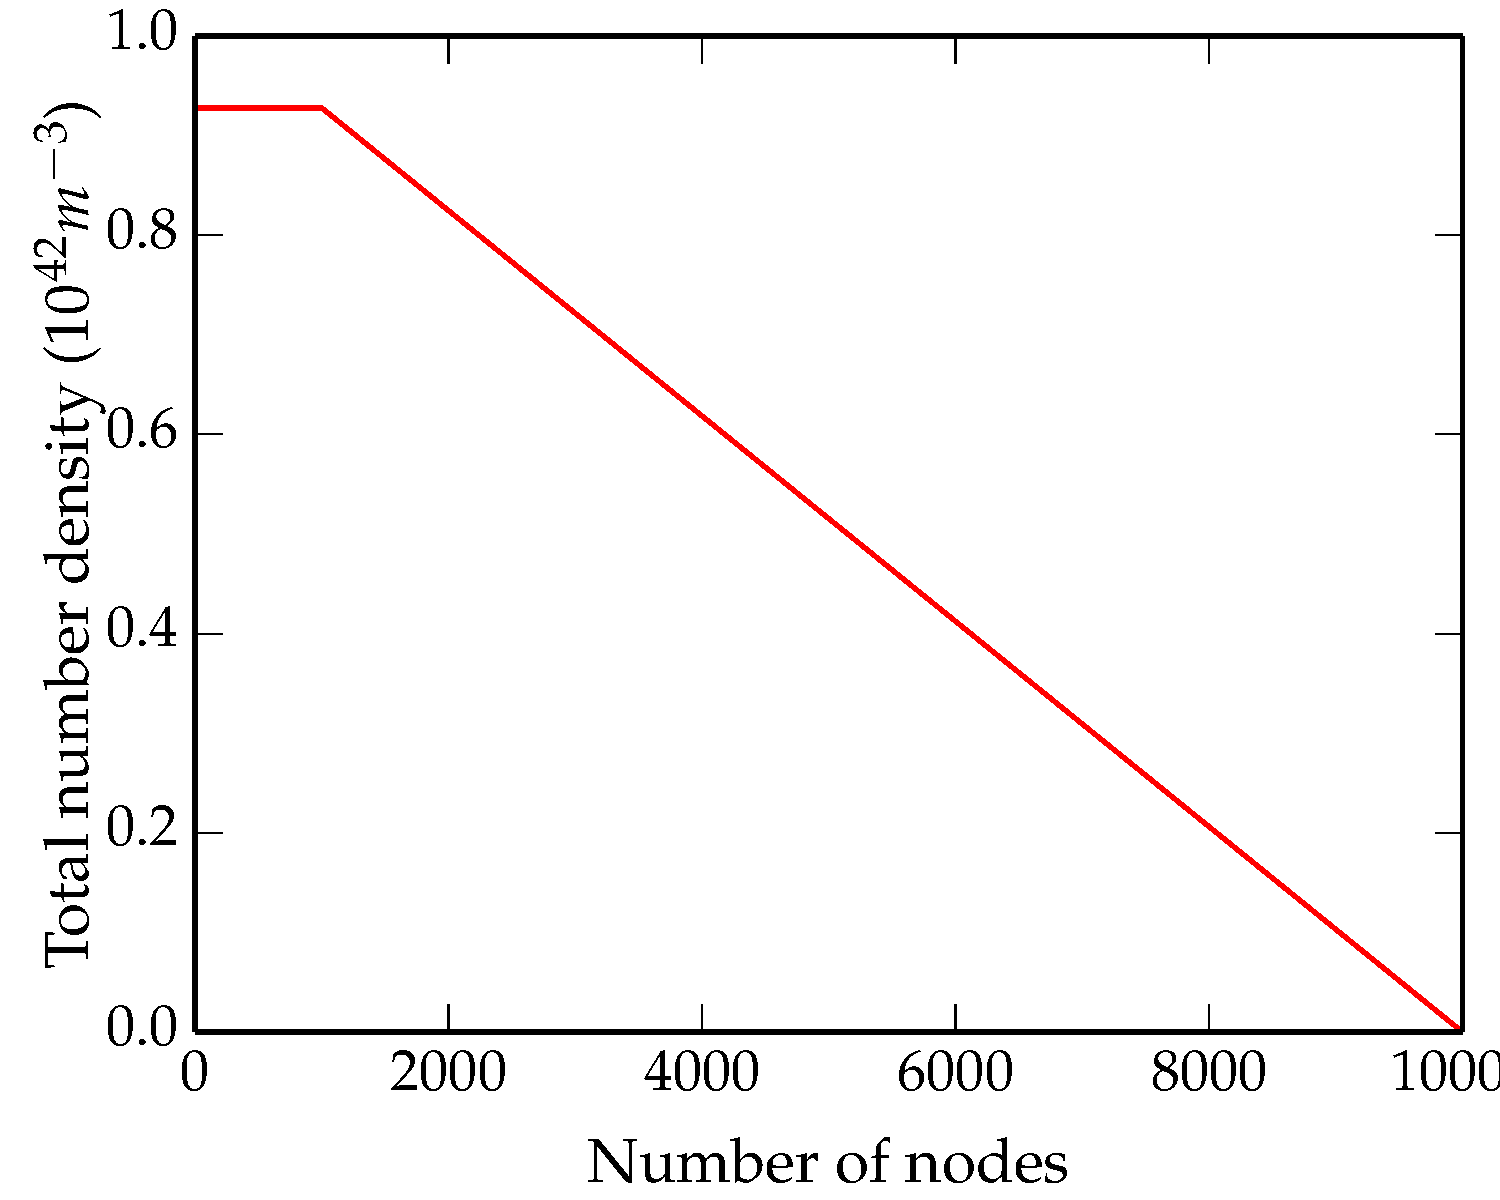
\includegraphics[width=0.5\textwidth]{EnergyDens}
	\caption{The number density calculated with different number of nodes of Legendre function.}
	\label{fig:EnergyDens}
\end{figure}

I don't know why the answer is not the same as in previous subsection, but, in figure \ref{fig:EnergyDens}, at least we can see the convergence.

\end{document}